\documentclass[journal]{IEEEtran}

% ---------- Engine & fonts ----------
\usepackage{iftex}
\ifXeTeX
  \usepackage{fontspec}
  \setmainfont{TeX Gyre Termes}
  \setsansfont{TeX Gyre Heros}
  \setmonofont{TeX Gyre Cursor}
\fi

% ---------- Packages ----------
\usepackage{graphicx}
\usepackage{amsmath,amssymb}
\usepackage{siunitx}
\usepackage{booktabs}
\usepackage[numbers,sort&compress]{natbib}
\usepackage{hyperref}
\usepackage{url}
\usepackage{tikz}
\usetikzlibrary{arrows.meta,positioning,fit}
\usepackage{pgfplots}
\pgfplotsset{compat=1.18}

% ---------- Helper: safe \input ----------
\makeatletter
\newcommand{\maybeinput}[1]{%
  \IfFileExists{#1}{\input{#1}}{\textit{[missing: #1]}}%
}
\makeatother

% ---------- Begin Document ----------
\begin{document}

\title{FeFET CMOS 0.18\,$\mu$m Integration Study}

% タイトル下に著者情報(肩書き・Email(半角)・GitHub)
\author{Shinichi~Samizo\\
\small Independent Semiconductor Researcher; Former Engineer at Seiko Epson Corporation\\
\small Email: \texttt{shin3t72@gmail.com}\quad GitHub: \url{https://github.com/Samizo-AITL}
}
\maketitle

% ================= Abstract & Index Terms =================
\begin{abstract}
\maybeinput{build/abstract_en.tex}
\end{abstract}

\begin{IEEEkeywords}
FeFET, HfZrO$_x$, 0.18\,$\mu$m CMOS, reliability, process integration
\end{IEEEkeywords}

% ================= Body =================
\section{Introduction}
\maybeinput{build/intro_en.tex}

% =========================================================
% Process Integration
% =========================================================
\section{Process Integration}

\subsection*{Baseline and Added Steps}
The ferroelectric (FE) gate stack is inserted after polysilicon definition. Additional process steps are minimized and summarized in Table~\ref{tab:masks}. Fig.~\ref{fig:flow} shows placement within the baseline.

% ---- Flow (TikZ, 2カラム幅で右切れ防止) ----
\begin{figure*}[t]
\centering
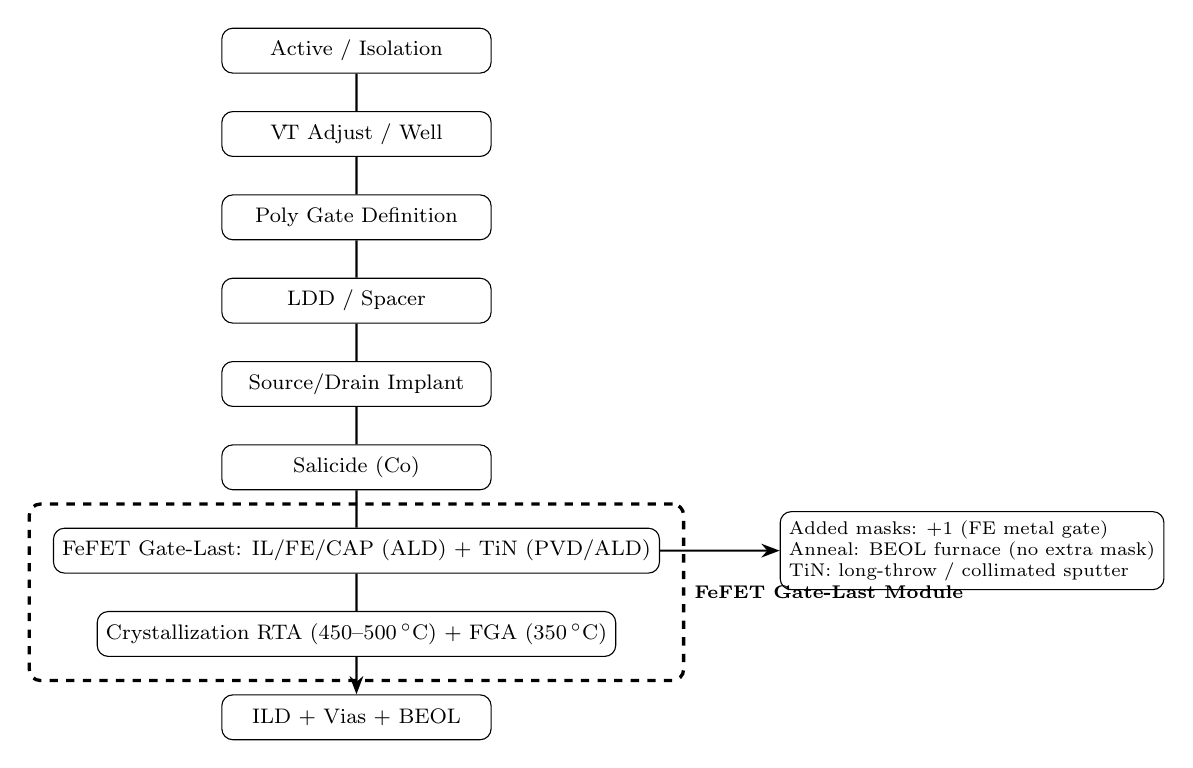
\begin{tikzpicture}[
  scale=0.95, every node/.style={transform shape},
  node distance=5mm,
  stage/.style={draw,rounded corners,minimum width=36mm,minimum height=6mm,align=center,font=\footnotesize},
  arr/.style={-{Stealth},thick},
  ann/.style={font=\scriptsize}
]
\node[stage] (act)  {Active / Isolation};
\node[stage,below=of act] (vt)  {V\!T Adjust / Well};
\node[stage,below=of vt]  (poly) {Poly Gate Definition};
\node[stage,below=of poly] (ldd)  {LDD / Spacer};
\node[stage,below=of ldd]  (imp)  {Source/Drain Implant};
\node[stage,below=of imp]  (sal)  {Salicide (Co)};
\node[stage,below=of sal]  (fegate)  {FeFET Gate-Last: IL/FE/CAP (ALD) + TiN (PVD/ALD)};
\node[stage,below=of fegate]  (rta)  {Crystallization RTA (450--500\,\si{\celsius}) + FGA (350\,\si{\celsius})};
\node[stage,below=of rta]  (ild)  {ILD + Vias + BEOL};
\draw[arr] (act) -- (vt) -- (poly) -- (ldd) -- (imp) -- (sal) -- (fegate) -- (rta) -- (ild);

\node[draw,dashed,very thick,rounded corners,fit=(fegate) (rta),inner sep=3mm,
      label={[ann]right:\textbf{FeFET Gate-Last Module}}] {};

\node[draw,rounded corners,align=left,font=\scriptsize,anchor=west,
      right=16mm of fegate] (note) {Added masks: +1 (FE metal gate)\\
Anneal: BEOL furnace (no extra mask)\\
TiN: long-throw / collimated sputter};
\draw[arr] (fegate.east) -- (note.west);
\end{tikzpicture}
\caption{Placement of the FeFET gate-last module in the 0.18\,$\mu$m CMOS baseline flow (vertical layout).}
\label{fig:flow}
\end{figure*}

% ---- Mask/step table ----
\begin{table}[t]
  \centering
  \caption{Added masks / process steps relative to baseline logic.}
  \label{tab:masks}
  \begin{tabular}{@{}lcc@{}}
    \toprule
    \textbf{Step} & \textbf{Mask} & \textbf{Comment}\\
    \midrule
    FE metal gate & +1 & Shared / reuse analog option route\\
    FE anneal     &  0 & Done in BEOL furnace (no extra mask)\\
    \bottomrule
  \end{tabular}
\end{table}

\subsection*{Device Stack}
TiN / Hf$_{0.5}$Zr$_{0.5}$O$_2$ (8--12\,nm, ALD) / Al$_2$O$_3$ IL (1--2\,nm) / p-Si.

\subsection*{Implementation Notes}
The 1.8\,V / 3.3\,V CMOS baseline was extended with an additional 1.8\,V FeFET option. FeFET devices are used as auxiliary elements for 1.8\,V SRAM macros, not as large-scale memory blocks. Although challenges remain regarding endurance, retention, TDDB, and yield, difficulty is reduced since large array scaling is not targeted. Integration is feasible within a legacy 0.18\,$\mu$m line by adding ALD; TiN can use existing barrier sputter (long-throw/collimated). The FeFET module is inserted after FEOL Co salicide and lamp anneal, requiring only one extra mask.

% =========================================================
% Experimental Conditions  (★重複を解消:この1回のみ)
% =========================================================
\section{Experimental Conditions}
Ferroelectric gate stacks were prepared with the following conditions:
\begin{itemize}
  \item Hf$_{0.5}$Zr$_{0.5}$O$_2$ thickness: 10\,nm (ALD deposition).
  \item Capacitor area: $100 \times 100\,\mu\mathrm{m}^2$.
  \item Gate voltage: $\pm 3$\,V, pulse width 1--1\,ms.
  \item Measurement frequency: 1\,kHz--1\,MHz.
  \item Equipment: Keysight B1500A semiconductor analyzer with Cascade probe station.
\end{itemize}

% =========================================================
% Reliability
% =========================================================
\section{Reliability}

% (図は既存の PGFPlots/TikZ 図を build/reliability_en.tex の前に配置してOK)
\begin{figure}[t]
\centering
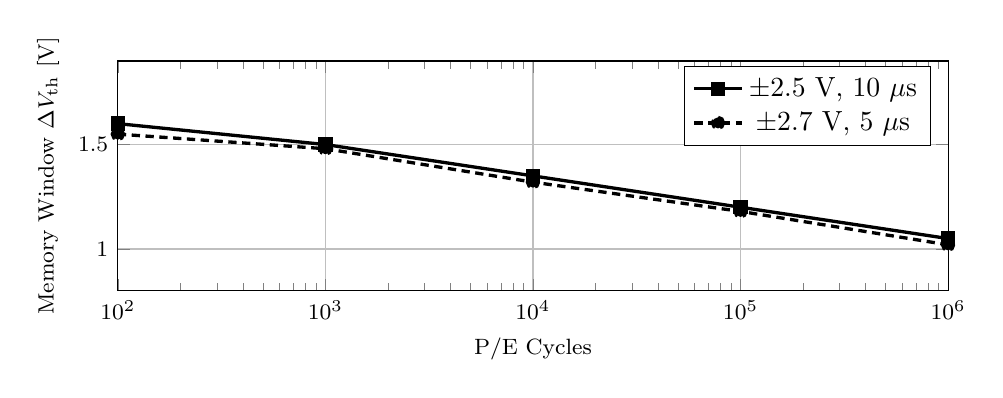
\begin{tikzpicture}
\begin{axis}[
  width=\columnwidth, height=45mm,
  xlabel={P/E Cycles}, ylabel={Memory Window $\Delta V_\mathrm{th}$ [V]},
  xmode=log, xmin=1e2, xmax=1e6, ymin=0.8, ymax=1.9,
  ymajorgrids, xmajorgrids, tick label style={font=\footnotesize}, label style={font=\footnotesize}
]
\addplot[very thick,mark=square*] coordinates {(1e2,1.6) (1e3,1.5) (1e4,1.35) (1e5,1.2) (1e6,1.05)};
\addlegendentry{$\pm 2.5$ V, 10 $\mu$s}
\addplot[densely dashed,very thick,mark=*] coordinates {(1e2,1.55) (1e3,1.48) (1e4,1.32) (1e5,1.18) (1e6,1.02)};
\addlegendentry{$\pm 2.7$ V, 5 $\mu$s}
\end{axis}
\end{tikzpicture}
\caption{Schematic endurance behavior of HZO-FeFETs in a 0.18\,$\mu$m flow.}
\label{fig:endurance}
\end{figure}

\begin{figure}[t]
\centering
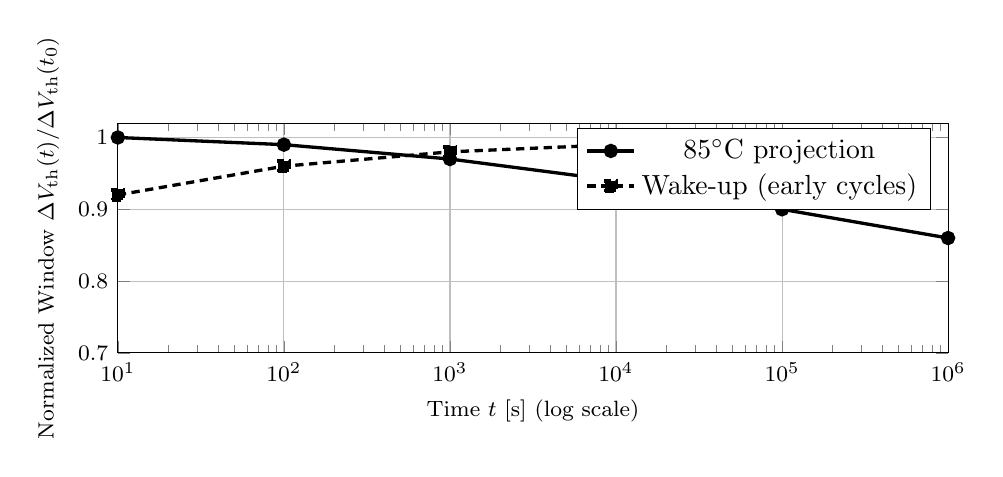
\begin{tikzpicture}
\begin{semilogxaxis}[
  width=\columnwidth, height=45mm,
  xmin=1e1, xmax=1e6, ymin=0.7, ymax=1.02,
  xlabel={Time $t$ [s] (log scale)}, ylabel={Normalized Window $\Delta V_\mathrm{th}(t)/\Delta V_\mathrm{th}(t_0)$},
  ymajorgrids, xmajorgrids, tick label style={font=\footnotesize}, label style={font=\footnotesize}
]
\addplot[very thick,mark=*] coordinates {(1e1,1.0) (1e2,0.99) (1e3,0.97) (1e4,0.94) (1e5,0.90) (1e6,0.86)};
\addlegendentry{$85^{\circ}$C projection}
\addplot[densely dashed,very thick,mark=square*] coordinates {(1e1,0.92) (1e2,0.96) (1e3,0.98) (1e4,0.99) (1e5,0.985)};
\addlegendentry{Wake-up (early cycles)}
\end{semilogxaxis}
\end{tikzpicture}
\caption{Retention (Arrhenius-projected) and early-cycle wake-up illustration.}
\label{fig:retention}
\end{figure}

\maybeinput{build/reliability_en.tex}

% =========================================================
% Conclusion(★重複を解消:この1回のみ)
% =========================================================
\section{Conclusion}
\maybeinput{build/conclusion_en.tex}

% ================= References =================
\bibliographystyle{IEEEtran}
\bibliography{refs}

% ================= Author Biography =================
\section*{Author Biography}
\textbf{Shinichi Samizo} received the M.S. degree in Electrical and Electronic Engineering from Shinshu University, Japan. He joined Seiko Epson Corporation in 1997, where he engaged in semiconductor device process development including 0.25--0.18\,$\mu$m CMOS, HV-CMOS, DRAM, FeRAM, and FinFET/GAA research. He also contributed to inkjet MEMS process development and thin-film piezo actuator design, leading to the productization of PrecisionCore printheads. His expertise covers semiconductor devices (logic, memory \mbox{[DRAM/FeRAM/SRAM]}, high-voltage mixed integration), inkjet actuators, and AI-based control education.

\end{document}
